\documentclass[sigconf]{acmart}

\usepackage{booktabs} % For formal tables
\usepackage{amsmath,amssymb}
% \usepackage{cite}   % importing cite is throwing errors for some reason
\usepackage{color}
\usepackage{enumerate}
\usepackage{multicol}

\usepackage{tikz}
\tikzset{
  treenode/.style = {shape=rectangle, rounded corners,
                     draw, align=center,
                     top color=white, bottom color=blue!20},
  root/.style     = {treenode, font=\Large, bottom color=red!30},
  env/.style      = {treenode, font=\ttfamily\normalsize},
  dummy/.style    = {circle,draw}
}

\usepackage{tikz-qtree}
\usepackage{tikz-qtree-compat}
\usetikzlibrary{positioning}
\usepackage{ textcomp }
% Get todos to render properly
\usepackage[obeyFinal]{easy-todo}

% Add package for ::= symbol, can't compile to pdf for some reason
% \usepackage{txfonts}

% Add package for well rendered quotations
\usepackage{dirtytalk}
\usepackage{hyperref}
\usepackage{graphicx}

\usepackage{lambda}

% correct bad hyphenation here
\hyphenation{op-tical net-works semi-conduc-tor}

% Copyright
%\setcopyright{none}
%\setcopyright{acmcopyright}
%\setcopyright{acmlicensed}
\setcopyright{rightsretained}
%\setcopyright{usgov}
%\setcopyright{usgovmixed}
%\setcopyright{cagov}
%\setcopyright{cagovmixed}


% DOI
\acmDOI{10.475/123_4}

% ISBN
\acmISBN{123-4567-24-567/08/06}

%Conference
\acmConference[Seattle'2017]{SIGCSE}{March 2017}{Seattle, Washington USA} 
\acmYear{2017}
\copyrightyear{2017}

\acmPrice{15.00}


\begin{document}
\title{A Domain Analysis of Data Structure and Algorithm Explanations in the Wild}


\author{Jeffrey Young} 
\affiliation{%
 \institution{Oregon State University}
 \department{School of EECS}
 \city{Corvallis} 
 \state{Oregon}
 \country{USA}}
\author{Eric Walkingshaw} 
\affiliation{%
 \institution{Oregon State University}
 \department{School of EECS}
 \city{Corvallis} 
 \state{Oregon}
 \country{USA}}
\todo{anonymize authors}


\begin{abstract}
  Explanations of data structures and algorithms are complex interactions of
  several notations, including natural language, mathematics, pseudocode, and
  diagrams. Currently, such explanations are created ad hoc using a variety of
  tools, and the resulting artifacts are static, reducing explanatory value. We
  envision a domain-specific language for developing rich, interactive
  explanations of data structures and algorithms. In this paper, we analyze this
  domain to sketch requirements for our language. We perform a grounded theory
  analysis, to generate a qualitative coding system for explanation artifacts
  collected online. We show that grounded theory provides a robust methodology
  for analyzing qualitative objects and that the resultant coding system forms
  the skeleton of a domain-specific language. This work is part of our effort to
  develop the paradigm of explanation-oriented programming, which shifts the
  focus of programming from computing results to producing rich explanations of
  how those results were computed.
  \todo{I want to say something here about using formal qualitative methods to
    expand the reach of computer science}
\end{abstract}

%
% The code below should be generated by the tool at
% http://dl.acm.org/ccs.cfm
% Please copy and paste the code instead of the example below. 
%
\todo{CCSXML}
\begin{CCSXML}
<ccs2012>
 <concept>
  <concept_id>10010520.10010553.10010562</concept_id>
  <concept_desc>Computer systems organization~Embedded systems</concept_desc>
  <concept_significance>500</concept_significance>
 </concept>
 <concept>
  <concept_id>10010520.10010575.10010755</concept_id>
  <concept_desc>Computer systems organization~Redundancy</concept_desc>
  <concept_significance>300</concept_significance>
 </concept>
 <concept>
  <concept_id>10010520.10010553.10010554</concept_id>
  <concept_desc>Computer systems organization~Robotics</concept_desc>
  <concept_significance>100</concept_significance>
 </concept>
 <concept>
  <concept_id>10003033.10003083.10003095</concept_id>
  <concept_desc>Networks~Network reliability</concept_desc>
  <concept_significance>100</concept_significance>
 </concept>
</ccs2012>  
\end{CCSXML}

\ccsdesc[500]{Computer systems organization~Embedded systems}
\ccsdesc[300]{Computer systems organization~Redundancy}
\ccsdesc{Computer systems organization~Robotics}
\ccsdesc[100]{Networks~Network reliability}


\todo{figure out keywords}
\keywords{ACM proceedings, \LaTeX, text tagging}

\maketitle

\section{Introduction}
\label{sec:intro}

Data structures and algorithms are at the heart of computer science and must be
explained to each new generation of students. A pressing question is: How can we
do this effectively?

In this paper, we focus on the \emph{artifacts} that constitute or support
explanations of data structures and algorithms (hereafter just ``algorithms''),
which can be shared and reused.
%
For verbal explanations, such as a lecture, the supporting artifact might be
the associated slides. For written explanations, the artifact is the
explanation as a whole, including the text and any supporting figures.
%
Explanation artifacts associated with algorithms are interesting because they
typically present a complex interaction among many different notations,
including natural language, mathematics, pseudocode, executable code, various
kinds of diagrams, animations, and more.


Currently, explanation artifacts for algorithms are created ad hoc using a
variety of tools and techniques, and the resulting explanations tend to be
static, reducing their explanatory value.
%
Although there has been a substantial amount of work on algorithm visualization~
\cite{Gloor92,Gloor97,HDS02, shaffer2010algorithm, HANSEN2002291, KANN1997223},
and tools exist for creating these kinds of supporting artifacts, there is no
good solution for creating integrated, multi-notational explanations as a whole.
Similarly, although some algorithm visualization tools provide a means for the
student to tweak the parameters or inputs to an algorithm to generate new
visualizations, they do not support creating cohesive interactive explanations
that correspondingly modify the surrounding explanation or that allow the
student to respond to or query the explanation in other ways.
%
To fill this gap, we envision a \emph{domain-specific language} (DSL) that
supports the creation of rich, interactive, multi-notational artifacts for
explaining algorithms.
%
The development of this DSL is part of a larger effort to explore the new
paradigm of \emph{explanation-oriented programming}, briefly described in
Section~ \ref{sec:back:xop}.


The intended users of the envisioned DSL are CS educators who want to create
\emph{interactive artifacts} to support the explanation of algorithms. These
users are experts on the corresponding algorithms, and also trained and skilled
programmers. The produced explanation artifacts might supplement a lecture or
be posted to a web page as a self-contained (textual and graphical)
explanation.
%
The DSL should support pedagogical methods directly through built-in
abstractions and language constructs. It should also support a variety of forms
of student interaction. For example, teachers should be able to define
equivalence relations enabling users to automatically generate variant
explanations~\cite{EW13jvlc}, to build in specific responses to anticipated
questions, and to provide explanations at multiple levels of abstraction.


This paper represents a formative step toward this vision. We conduct a
\emph{qualitative analysis} of our domain in order to determine the form and
content of the explanation artifacts that educators are already creating.
%
We base our analysis on an established qualitative research method called
\emph{grounded theory} in order to better understand how well existing artifacts
explain complex topics


More specifically, we collect 15 explanation artifacts from the internet,
consisting of only lecture notes that explain two algorithms and one
data structure commonly covered in undergraduate computer science courses:
Dijkstra's shortest path algorithm~\cite[pp.~137--142]{KT06}, merge sort
\cite[210--214]{KT06}, and AVL trees \cite[pp.~458--475]{KnuthArt3}.
%
We analyze these artifacts through the application of grounded theory,
\todo{cite Strauss and Corbin on first grounded theory paper} a formal method
for analyzing qualitative data that originated in sociological research. Through
the application of grounded theory, we develop a coding system that captures
the structure of explanation for each document. An overview of the coding system
is given in Section\todo{create grounded theory overview section}.

% We analyze these artifacts by applying a classic pedagogical theory by Bellack
% et al.~\cite{bellack1966language} that describes the patterns of language used
% in the process of teaching. Bellack et al.\ define a typology for coding
% transcripts of teacher and student verbalizations during teaching. An overview
% of the typology is given in Section~\ref{sec:back:typ}.


This paper makes the following contributions:
%
\begin{enumerate}[C1.]

\item \label{contrib:method}
  We provide a case study on analyzing \emph{qualitative data} through the
  application of a formal research method \emph{grounded theory}, that is not
  part of the computer science parlance.

\item \label{contrib:data}
%
We provide a coded qualitative data set of explanation artifacts, using the
system defined in C\ref{contrib:codes} applied to our sample of 15 collected
explanation artifacts (Section~\ref{sec:exp:data}).

\item \label{contrib:codes}
%
\todo{decide if we need to split this contribution up}
We provide a coding system for analyzing \emph{explanation artifacts} in the
form of lecture notes, and we show that through the application of the coding
system, each such artifact forms a tree structure, which we have termed a
\emph{explanation tree}.


\item \label{contrib:dsl}
%
  We describe how a coding system grounded in data can directly provide a
  semantics basis for a DSL and argue for the advantages of such an approach
  (Section~\ref{sec:res:dsl}).
%
\end{enumerate}

\noindent

\section{Background}
\label{sec:back}

\begin{figure}
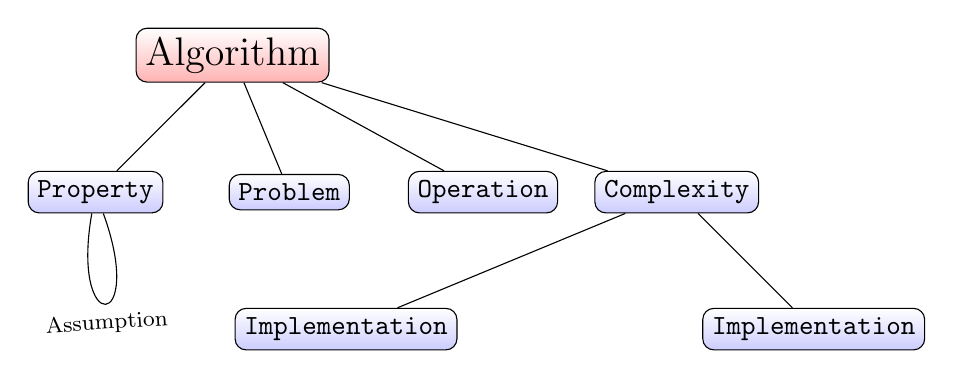
\begin{tikzpicture}
  [
    grow                    = right,
    node distance           = 7em,
    edge from parent/.style = {draw, -latex},
    every node/.style       = {font=\footnotesize},
    sloped
  ]
  \node [root] (0) {Algorithm};
  \node [env] (1) [below left of=0] {Property};
  \node [env] (2) [right of=1] {Problem};
  \node [env] (3) [right of=2] {Operation};
  \node [env] (4) [right of=3] {Complexity};
  \node [env] (5) [below left of=3] {Implementation};
  \node [env] (6) [below right of=4] {Implementation};

  \path [-]
    (0) edge (1)
    (0) edge (2)
    (0) edge (3)
    (0) edge (4)
    (4) edge (5)
    (4) edge (6)
    (1) edge [below, out=290, in=260, looseness=8, distance=1.6cm]
        node [swap] {Assumption} (1);
  
\end{tikzpicture}
\todo{Fix this caption, and figure, this was just proof of concept}
\caption{Explanation Tree for Dijkstra's 009}
\label{fig:djk-tree}
\end{figure}

\bibliography{XOPbib.bib,eric.bib}
\bibliographystyle{ACM-Reference-Format}

\end{document}
